% `template.tex', a bare-bones example employing the AIAA class.
%
% For a more advanced example that makes use of several third-party
% LaTeX packages, see `advanced_example.tex', but please read the
% Known Problems section of the users manual first.
%
% Typical processing for PostScript (PS) output:
%
%  latex template
%  latex template   (repeat as needed to resolve references)
%
%  xdvi template    (onscreen draft display)
%  dvips template   (postscript)
%  gv template.ps   (onscreen display)
%  lpr template.ps  (hardcopy)
%
% With the above, only Encapsulated PostScript (EPS) images can be used.
%
% Typical processing for Portable Document Format (PDF) output:
%
%  pdflatex template
%  pdflatex template      (repeat as needed to resolve references)
%
%  acroread template.pdf  (onscreen display)
%
% If you have EPS figures, you will need to use the epstopdf script
% to convert them to PDF because PDF is a limmited subset of EPS.
% pdflatex accepts a variety of other image formats such as JPG, TIF,
% PNG, and so forth -- check the documentation for your version.
%
% If you do *not* specify suffixes when using the graphicx package's
% \includegraphics command, latex and pdflatex will automatically select
% the appropriate figure format from those available.  This allows you
% to produce PS and PDF output from the same LaTeX source file.
%
% To generate a large format (e.g., 11"x17") PostScript copy for editing
% purposes, use
%
%  dvips -x 1467 -O -0.65in,0.85in -t tabloid template
%
% For further details and support, read the Users Manual, aiaa.pdf.


% Try to reduce the number of latex support calls from people who
% don't read the included documentation.
%
\typeout{}\typeout{If latex fails to find aiaa-tc, read the README file!}
%


\documentclass[]{aiaa-tc}% insert '[draft]' option to show overfull boxes
\usepackage{mathtools}
\usepackage{amsmath}
\usepackage{amssymb}
\usepackage{newlfont}
\usepackage{notoccite}
\usepackage[nomarkers,figuresonly]{endfloat}

 \title{A Decoupled Method for the Roe FDS Scheme in the Reacting Gas Path of FUN3D}

 \author{
  Kyle B. Thompson%
    \thanks{NASA Pathways Intern, Aerothermodynamics Branch, AIAA Student Member.}
  \ and Peter A. Gnoffo\thanks{Senior Research Engineer, Aerothermodynamics Branch, AIAA Fellow.}\\
  {\normalsize\itshape
   NASA Langley Research Center, Hampton, VA, 23681-2199}\\
 }

 % Data used by 'handcarry' option if invoked
 \AIAApapernumber{YEAR-NUMBER}
 \AIAAconference{Conference Name, Date, and Location}
 \AIAAcopyright{\AIAAcopyrightD{YEAR}}

 % Define commands to assure consistent treatment throughout document
 \newcommand{\eqnref}[1]{(\ref{#1})}
 \newcommand{\class}[1]{\texttt{#1}}
 \newcommand{\package}[1]{\texttt{#1}}
 \newcommand{\file}[1]{\texttt{#1}}
 \newcommand{\BibTeX}{\textsc{Bib}\TeX}

\begin{document}

\maketitle

\begin{abstract}
In this paper, we describe an approach for decoupling the species continuity equations from the mixture continuity, momentum, and total energy equations for the Roe flux difference splitting scheme.  Utilizing aspects of the implicit system, the flow solver can be made significantly more efficient, with very little penalty on overall scheme robustness.  Most importantly, the computational cost of the point implicit relaxation is shown to scale linearly with the number of species for the decoupled system, whereas the fully coupled approach scales quadratically.  We show that solving the implicit system in a decoupled fashion significantly reduces the cost in wall time and memory in comparison to the fully coupled approach.
\end{abstract}

\section*{Nomenclature}

\begin{tabbing}
  XXXXXXXXX \= \kill% this line sets tab stop
  $A,\ A_d,\ A_m$ \> Jacobian Matricies \\
  $a$ \> Speed of sound $m/s$ \\
  $\mathbf{b}$ \> Residual vector \\
  $c_s$ \> Species $s$ mass fraction \\
  $C$ \> Decoupled scheme chemical source term jacobian \\
  $D$ \> Decomposed diagonal jacobian matrix \\
  $dv_1,\ dv_2,\ dv_3$ \> Eigenvector components \\
  $e_s$ \> Internal energy of species $s$ \\
  $E$ \> Total Energy \\
  $F_\rho'$\> Decoupled scheme mixture mass flux \\
  $F_{\rho_s}'$\> Decoupled scheme mass flux of species $s$ \\
  $\mathbf{F},\ \mathbf{F}',\ \mathbf{\hat{F}}$ \> Flux vectors \\
  $N_{nodes}$ \> Number of nodes \\
  $N_{nz}$ \> Number of non-zero off-diagonal entries in jacobian \\
  $O$ \> Decomposed off-diagonal jacobian matrix \\
  $p$ \> Pressure, $N/m^2$ \\
  $\mathbf{R},\ \mathbf{L}$ \> Right and left eigenvectors \\
   $R_\rho$ \> Decoupled scheme constraint \\
  $\mathbf{S}$ \> Face normal vector, $m^2$\\
  $\mathbf{U},\ \mathbf{U}',\ \mathbf{\hat{U}}$ \> Conservative variable vectors \\
  $\overline{U}$ \> Normal velocity, $m/s^2$ \\
  $u,\ v,\ w$ \> Components of velocity, $m/s$ \\
  $V$ \> Decoupled variables vector \\
  $w$ \> Roe scheme weighting factor \\
  $\mathbf{\hat{V}}$ \> Cell volume, $m^3$ \\
   $\mathbf{W}$ \> Chemical source term vector \\
   \\
   $\rho$ \> Mixture density $kg/m^3$ \\
   $\rho_s$ \> Species $s$ density $kg/m^3$ \\
   $\lambda_1,\ \lambda_2,\ \lambda_3$ \> Acoustic and convective eigenvalues \\
    $\lambda^-,\ \lambda^+$ \> Species flux effective eigenvalues \\
    $\Lambda$ \> Diagonal eigenvalue matrix \\
   \\

  \textit{Superscript}\\
  $n, n+1$ \> Time level \\
  $R,\ L$ \> Right and left state quantities \\
 \end{tabbing}

\section{Introduction}

The usability of hypersonic solvers on complex geometries is often limited by the extreme problem size associated with high energy physics.  The additional equations required in reacting gas simulations lead to large jacobians that scale quadratically in size to the number of governing equations.  This leads to a significant increase in memory required to store the flux linearizations and the computational cost of the point solver.  As reacting gas CFD solvers are used to solve increasingly more complex problems, this onerous quadratic scaling of computational cost and jacobian size will ultimately surpass the limits of hardware and time constraints on achieving a flow solution.

The proposed method is based heavily upon the work of Candler et al.\cite{candler}, where the quadratic scaling between the cost of solving the implicit system and the addition of species mass equations can be reduced to that of a linear scaling by decoupling the species mass equations from the mixture mass, momentum, and energy equations and solving the two decoupled systems sequentially.  In the aforementioned work, the scheme was derived for a modified form of the Steger-Warming flux vector splitting method\cite{MacCormack}, whereas the work presented here is derived for Roe flux difference splitting (FDS) scheme.

A primary motivator for the presented work is to prepare for the implementation of an adjoint capability in a reacting gas solver.  This is an extremely challenging problem, and a significant hardship is deriving exact jacobians for a reacting gas system.  A beneficial side effect of decoupled the system is the simplification of deriving exact jacobians for the Roe flux difference splitting scheme.  By decoupling the species equations, the mixture mass, moment, and energy flux jacobians can be easily derived\cite{Nishikawa}, using a weighting scheme to correct for the non-uniqueness of the pressure linearization\cite{Shuen}.  For the decoupled species fluxes we derive an exact linearization in the presented work.

\section{Background: Fully-Coupled Point Implicit Method}

All work presented here is for the inviscid conservation equations, but can be extended to include viscous terms.  For an inviscid, multi-species mixture, the governing equations in vector form are:
%
\begin{equation}
	\label{inv_flux_vec}
	\frac{\partial \mathbf{U}}{\partial t}
	+ \nabla\cdot \mathbf{F} = \mathbf{W}
\end{equation}
%
 or, in finite volume form:
 %
\begin{equation}
	\label{inv_flux_fv}
	\frac{\partial \mathbf{U}}{\partial t}
	 + \frac{1}{V}\sum\limits_{f}(\mathbf{F}\cdot\mathbf{S}) = \mathbf{W}
 \end{equation}
 %
summing over all faces in the domain, with V being the cell volume and $\mathbf{S}$ being the face outward normal vector.  The vectors of conserved variables and fluxes are:
%
\begin{equation}
	\begin{matrix}
	\mathbf{U}=\begin{pmatrix}
   		\rho_1\\
		\vdots \\
		\rho_{ns} \\
		\rho u \\
		\rho v \\
		\rho w \\
		\rho E \\
	\end{pmatrix},      &
 	\mathbf{F} = \begin{pmatrix}
		\rho_1  \overline{U} \\
		\vdots \\
		\rho_{ns} \overline{U} \\
		\rho u \overline{U} + p s_x\\
		\rho u \overline{U} + p s_y\\
		\rho u \overline{U} + p s_z\\
		(\rho E + p) \overline{U} \\
	\end{pmatrix}
	\end{matrix}
 \end{equation}
 %
 Where $\overline{U}$ is the outward pointing normal velocity and $\rho E$ is the total energy of the mixture, defined as:
 %
 \begin{equation}
 	E = \sum{\rho_s e_s} + \frac{u^2+v^2+w^2}{2}
\end{equation}
%
where $e_s$ is the internal energy of species $s$.  Using the Roe FDS scheme the numerical fluxes can be expressed as follows:
%
\begin{equation}
	\mathbf{F}^f=\frac{\mathbf{F}(\mathbf{U}^L)+\mathbf{F}(\mathbf{U}^R)}{2}-\frac{1}{2}\mathbf{R}\Lambda \mathbf{L}
\end{equation}
%
Where $\Lambda$ is the diagonal eigenvalue matrix, and $\mathbf{R}$ and $\mathbf{L}$ are the right and left eigenvectors, respectively.  We now linearize the flux and the source term vectors as:
%
\begin{equation}
	\begin{matrix}
		\mathbf{F}^{n+1} \approx \mathbf{F}^n+\frac{\partial \mathbf{F}}{\partial \mathbf{U}}\delta\mathbf{U}^n \\
		\\
		\mathbf{W}^{n+1} \approx \mathbf{W}^n+\frac{\partial \mathbf{W}}{\partial \mathbf{U}}\delta\mathbf{U}^n \\
	\end{matrix}
\end{equation}
%
where $\delta\mathbf{U}^n = \mathbf{U}^{n+1}- \mathbf{U}^{n}$.  Using an implicit time integration, the implicit scheme becomes:
%
\begin{equation}
	\frac{\mathbf{\delta U}^n}{\Delta t}+\frac{1}{V}\sum\limits_{f}(\frac{\partial \mathbf{F}}{\partial \mathbf{U^L}}\delta\mathbf{U}^L
	+\frac{\partial \mathbf{F}}{\partial \mathbf{U^R}}\delta\mathbf{U}^R)^n - \frac{\partial \mathbf{W}}{\partial \mathbf{U}}\delta\mathbf{U}^n
	= -\frac{1}{V}\sum\limits_{f}(\mathbf{F}\cdot\mathbf{S})^n + \mathbf{W}^n
\end {equation}
%
or, put more simply:
%
\begin{equation}
	A\delta\mathbf{U}^n = \mathbf{b}
\end{equation}
%
where $A$ is the jacobian matrix, and $\mathbf{b}$ is the residual vector.  For a point implicit relaxation scheme the jacobian matrix can be split into its diagonal and off-diagonal elements, with the latter moved to the RHS as such:
%
\begin{equation}
\label{decomp_jac}
	A=O+D
\end{equation}
%
Each matrix element is a square $(ns+4)\times(ns+4)$ matrix.  One method of solving this system is a Red-Black Gauss-Seidel scheme, where matrix coefficients with even indices are updated first and, subsequently, the coefficients with odd indices are updated.  This enables better vectorization in solving the linear system.  A key point here is the matrix multiplication of the elements of the decomposed $A$ matrix is a quadratic operation; thus, the cost of solving the implicit system scales quadratically with the number of equations being solved.

The addition of viscous terms does not change the form of the system and results in dense matrices being added to the jacobian matrix, $A$.

\section{Background: Decoupled Point Implicit Method}

By replacing the species mass equations with a single mixture equation and separating the mixture equations from the species mass equations, the conserved variables become:
%
\begin{equation}
	\begin{matrix}
		\mathbf{U}'=\begin{pmatrix}
			\rho \\
			\rho u \\
			\rho v \\
			\rho w \\
			\rho E
		\end{pmatrix} &
		\mathbf{\hat{U}}=\begin{pmatrix}
			\rho_1 \\
			\vdots \\
			\rho_{ns}
		\end{pmatrix}
	\end{matrix}
\end{equation}
%
Solving for the flux is now done in two sequential steps.  The mixture fluxes are first solved as:
%
\begin{equation}
	\frac{\partial \mathbf{{U}'}}{\partial t}
	 + \frac{1}{V}\sum\limits_{f}(\mathbf{F}'\cdot\mathbf{S}) = 0
 \end{equation}
 %
 Followed by the species fluxes
%
\begin{equation}
	\frac{\partial \mathbf{\hat{U}}}{\partial t}
	 + \frac{1}{V}\sum\limits_{f}(\mathbf{\hat{F}}\cdot\mathbf{S}) = \mathbf{\hat{W}}
 \end{equation}
 %
The point relaxation proceeds using Red-Black Gauss-Seidel to update the conserved variables in $\mathbf{U}'$ and all associated auxiliary variables, such as temperature, pressure, speed of sound, etc.  This is done holding the thermo-chemical state constant, and will always result in the relaxation of a 5-equation system.
 
 The solution of the species mass equations takes a different form.  Based on the work of Candler et al.\cite{candler} the decoupled variables can be rewritten in terms of mass fraction, as follows:
 %
 \begin{equation}
 	\delta \mathbf{\hat{U}}^n
	= \rho^{n+1}\mathbf{\hat{V}}^{n+1}-\rho^n\mathbf{\hat{V}}^n
	= \rho^{n+1} \delta \mathbf{\hat{V}}^n + \mathbf{\hat{V}}^n \delta \rho^n
\end{equation}
 %
 where $\mathbf{\hat{V}}=(c_1,\hdots,c_{ns})^T$, and $c_s=\rho_s/\rho$ the mass fraction of species $s$.  While the derivation of the species mass equations is different from that of the Steger-Warming FVS scheme proposed by Candler et al.\cite{candler}, the final result takes a similar form: 
%
\begin{gather}
	\hat{F}_{\rho_s} = c_s F'_\rho+(c_s^L-\tilde{c}_s)\rho^L\lambda^+ + (c_s^R-\tilde{c}_s)\rho^R\lambda^- \label{dc_flux}
\end{gather}
%
where $F_\rho'$ is the total mass flux computed previously using all $\mathbf{U}'$ variables.  Likewise, linearizing the species mass fluxes with respect to the $\mathbf{\hat{V}}$ variables yields:
%
\begin{align}
	\mathbf{\hat{F}}^{n+1} &= \mathbf{\hat{F}}^n
	+\frac{\partial \mathbf{\hat{F}}}{\partial \mathbf{\hat{V}}^L}\delta \mathbf{\hat{V}}^L
	+\frac{\partial \mathbf{\hat{F}}}{\partial \mathbf{\hat{V}}^R}\delta \mathbf{\hat{V}}^R \\
	\frac{\partial \mathbf{\hat{F}}}{\partial \mathbf{\hat{V}}^L} &= wF_\rho+(1-w)\rho^L\lambda^+ - w\rho^R\lambda^- \\
	\frac{\partial \mathbf{\hat{F}}}{\partial \mathbf{\hat{V}}^R} &= (1-w)F_\rho+(w-1)\rho^L\lambda^+ + w\rho^R\lambda^- \label{d_last}
\end{align}
%
A full derivation of Eq.s~(\ref{dc_flux}-\ref{d_last}) is included in Appendix A.  The chemical source term is evaluated with the $\mathbf{U}'$ variables, and the linearization is carried out as:
%
\begin{equation}
	\mathbf{\hat{W}}^{n+1} = \mathbf{\hat{W}}^n+\frac{\partial \mathbf{\hat{W}}}{\mathbf{U}}\bigg|_{\mathbf{U}'}
	\frac{\partial \mathbf{U}}{\partial \mathbf{\hat{V}}}
\end{equation}
%
For simplicity of notation, we define:
%
\begin{equation}
C = \frac{\partial \mathbf{\hat{W}}}{\mathbf{U}}\bigg|_{\mathbf{U}'}
	\frac{\partial \mathbf{U}}{\partial \mathbf{\hat{V}}}
\end{equation}
%
The decoupled system to be solved becomes:
%
\begin{gather}
	\begin{split}
	\rho^{n+1}&\frac{\mathbf{\delta \hat{V}}^n}{\Delta t}+\frac{1}{V}\sum\limits_{f}(\frac{\partial \mathbf{\hat{F}}}{\partial \mathbf{\hat{V}}^L}\delta 	\mathbf{\hat{V}}^L +\frac{\partial \mathbf{\hat{F}}}{\partial \mathbf{\hat{V}}^R}\delta \mathbf{\hat{V}}^R)^{n, n+1}
	- C^{n, n+1}\delta\mathbf{V}^n \\
	&= -\frac{1}{V}\sum\limits_{f}(\mathbf{\hat{F}}^{n,n+1}\cdot\mathbf{S}) + \mathbf{W}^{n, n+1}
	-\mathbf{\hat{V}}^n\frac{\delta \rho^n}{\Delta t} - R_\rho
	\end{split} \\
 	R_\rho = -\frac{1}{V}\sum\limits_{f}{\sum\limits_{s}{(\hat{F}_{\rho_s}^{n,n+1}\cdot\mathbf{S})}}
\end {gather}
%
where $R_\rho$ is included to preserve the constraint that the mass fractions sum to unity, i.e. 
$\sum\limits_{s}{c_s}=1, \quad \sum\limits_{s}{\delta c_s}=1$.

\section{Cost and Memory Savings of the Decoupled Implicit Problem}

In decoupling the species equations, the most significant savings comes from the source term linearization being purely node-based\cite{gnoffo-tp}.  Solving the mean flow equations is conducted in the same manner as the fully coupled system, where all entries in the jacobian $A_m$ are $5\times5$ matrices.  For the decoupled implicit system, all entries in the jacobian $A_d$ are $ns \times ns$ matrices.  Because there is no interdependence of species, except through the chemical source term, all contributions due to linearizing the convective flux are purely diagonal $ns \times ns$ matrices.  Via Eq.~(\ref{decomp_jac}), we decompose $A_d$ into its diagonal and off-diagonal elements, resulting in the following linear system:
%
\begin{equation}
\label{dc_sys}
	\begin{pmatrix}
		\Box & & \\
		& \ddots & \\
		& & \Box
	\end{pmatrix}
	\begin{pmatrix}
		\delta \hat{V_1} \\
		\vdots \\
		\delta \hat{V}_{nodes}
	\end{pmatrix} = b -
	\begin{pmatrix}
		0 & & \diagdown \\
		& \ddots & \\
		\diagdown & & 0
	\end{pmatrix}
	\begin{pmatrix}
		\delta \hat{V_1} \\
		\vdots \\
		\delta \hat{V}_{nodes}d
	\end{pmatrix}
\end{equation}
%
where $\Box$ represents a dense $ns \times ns$ matrix, and $\diagdown$ represents a diagonal matrix.  Thus, the non-zero entries in the off-diagonal matrix can be reduced from diagonal matrices to vectors, reducing the rank of the overall matrix by 1.  This results in significant savings in both cost and memory, as the only quadratic operation left in solving the implicit system is dealing with the diagonal entries in the jacobian.  Because the off-diagonal entries significantly outnumber of the diagonal entries, we can expect nearly linear scaling in cost with the number of species.  Utilizing compressed row storage\cite{George} for the off-diagonal entries, the relative memory savings in the limit of a large number of species for the jacobian is given by:
%
\begin{equation}
\label{mem_req_eq}
\begin{split}
	Relative\ Memory\ Cost &= \frac{size(A_d)}{size(A_m)} \\
	&= \lim_{ns\to\infty} \frac{(ns^2+5^2)(N_{nodes})+(ns+5^2)(N_{nz})}{(ns+4)^2(N_{nodes}+N_{nz})} \\
	&= \frac{N_{nodes}}{N_{nodes} + N_{nz}}
\end{split}
\end{equation}
%
Where $N_{nodes}$ is the number of nodes, and $N_{nz}$ is the number of non-zero off-diagonal entries stored using compressed row storage. For a structured grid, each node has 6 neighbors in 3D, i.e. $N_{nz} = 6N_{nodes}$; therefore, we can expect the jacobian memory required to decrease by a factor of 7 using this decoupled scheme. Interestingly, for a grid that is not purely hexahedral, $N_{nz} > 6N_{nodes}$, making this decoupled scheme even more efficient for unstructured grids than structured grids.

\section{Results}

The proposed decoupled scheme has been implemented in the NASA Langley unstructured grid solver FUN3D\cite{FUN3D}, as well as the traditional, fully coupled approach.  To demonstrate the improved efficiency in cost and memory required utilizing the decoupled scheme, and that both the fully coupled and decoupled approachhes converge to the same result, a grid convergence study was conducted on a simple hemisphere geometry (radius 0.5 m).  A 50 x 50, 100 x 100, and 200 x 200 family of grids were adapted using the line adaptation capability in FUN3D to produce well-aligned grids that approximate a true coarsening of the finest grid level.  The free stream conditions used were $V_{\infty} = 5000\ m/s$, $\rho_{\infty}=0.001\ kg/m^3$, $T_\infty = 200\ K$.  Several chemical kinetics models were used, including a 5-species model with 5 reactions, an 11-species model with 22 reactions, and an 18-species model with 29 reactions. 

\subsection{Comparison of Solution}

Most important is that the decoupled and fully coupled scheme give nearly identical converged solutions.  To quantitatively assess this, we compare the predicted surface pressure, surface temperature, the species composition on the stagnation line for both schemes.  Figures \ref{surf_press} through  \ref{stag_line} show that the predicted quantities on the on the 100 x 100 grid. All results are indeed nearly identical, with temperature and pressure matching discretely to 8 digits and the species mass fractions on the stagnation line matching to 4 digits.  This difference was observed to be reduced slightly more on the finest grid level of 200 x 200.
%
\begin{figure}
\begin{center}
\includegraphics{surface_pressure}
\caption{Pressure on Hemisphere Surface}
\label{surf_press}
\end{center}
\end{figure}
%
\begin{figure}
\begin{center}
\includegraphics{surface_temperature}
\caption{Temperature on Hemisphere Surface}
\label{surf_temp}
\end{center}
\end{figure}
%
\begin{figure}
\begin{center}
\includegraphics{stag_line_mf}
\caption{Species Mass Fractions on the Hemisphere Stagnation Line}
\label{stag_line}
\end{center}
\end{figure}

\subsection{Memory Cost}

In order to determine the required memory of the decoupled scheme in comparison to the fully coupled scheme, a convergence study was conducted using Valgrind\cite{valgrind} to determined the memory actually allocated by FUN3D for an increasing number of species.  
%
\begin{figure}
\begin{center}
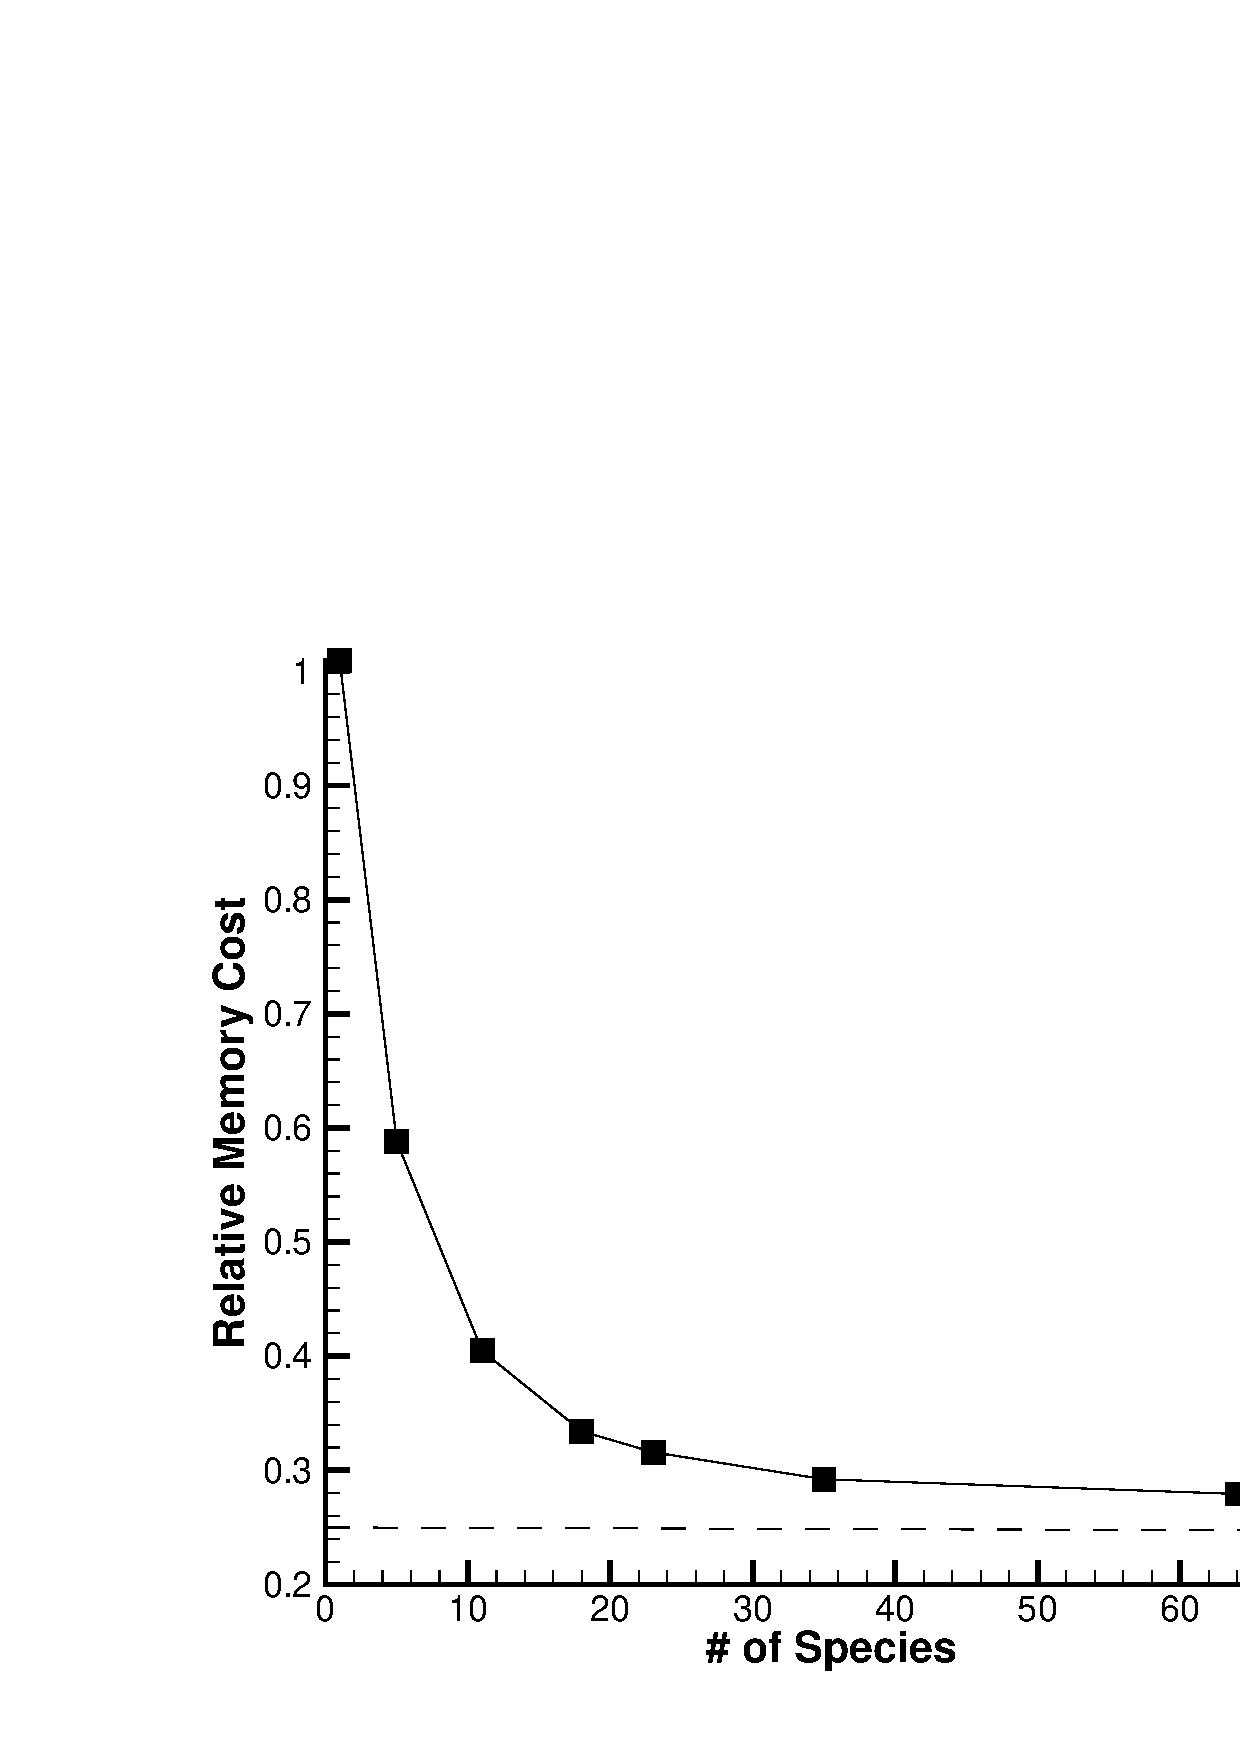
\includegraphics{mem_req}
\caption{Memory Required Convergence Study}
\label{mem_req}
\end{center}
\end{figure}
%
Figure \ref{mem_req} shows the relative memory cost converges asymptotically to $\sim 0.25$, which is nearly twice the predicted value of 1/7.  For the implementation of FUN3D this is actually correct, because the off-diagonal entries are reduced from double precision to single precision.  Starting from Eq.~(\ref{mem_req_eq}), for a structured grid (as is the case here) where each node has 6 neighbors, the relative memory cost come to:
%
\begin{equation}
	Relative\ Memory\ Cost = \frac{N_{nodes}}{N_{nodes} + N_{nz}} = \frac{N_{nodes}}{N_{nodes} + (6N_{nodes}/2)}=\frac{1}{4}
\end{equation}
%
thus, the relative memory saved by using the decoupled scheme correctly approaches a factor of 1/4.  It should be noted that the additional species in the 35-species and 64-species cases were chosen arbitrarily, since jacobian size is only dependent on the number of species, not the mixture composition.

\subsection{Computational Cost}

As stated before, the cost of solving the decoupled implicit system should scale approximately linearly with the number of species, whereas the fully coupled problem should scale quadratically.  Figure \ref{lsolve_speedup} shows this to be true for the hemisphere test case.
%
\begin{figure}
\begin{center}
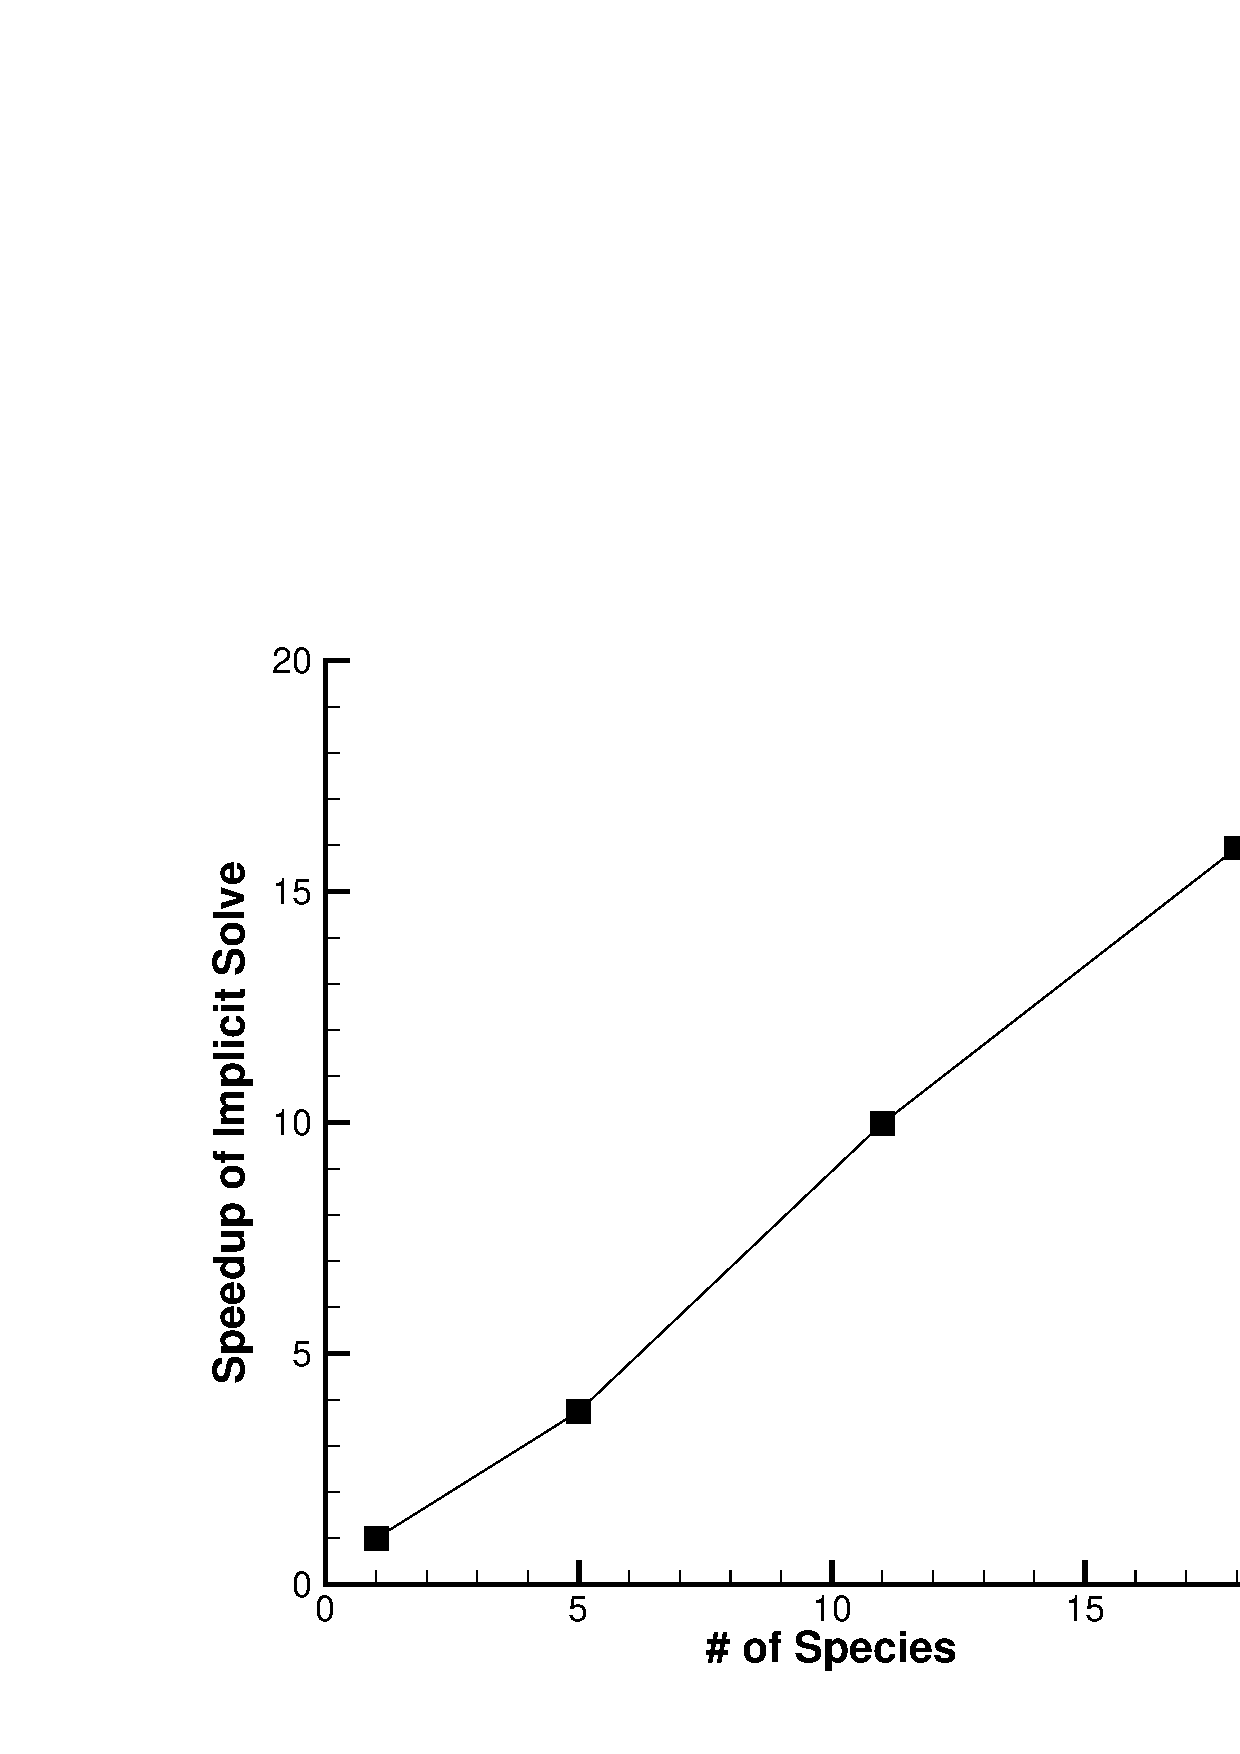
\includegraphics{linear_solve_speedup}
\caption{Relative Speedup of Implicit Solve for the Decoupled Scheme wrt the Fully Coupled Scheme}
\label{lsolve_speedup}
\end{center}
\end{figure}
%
Figure \ref{overall_speedup} shows the total speed up of the problem to be less than that of the just the linear solve.   This is to be expected, as there are many other factors that scale with the number of species, especially calculating the species source term and its linearization.
%
\begin{figure}
\begin{center}
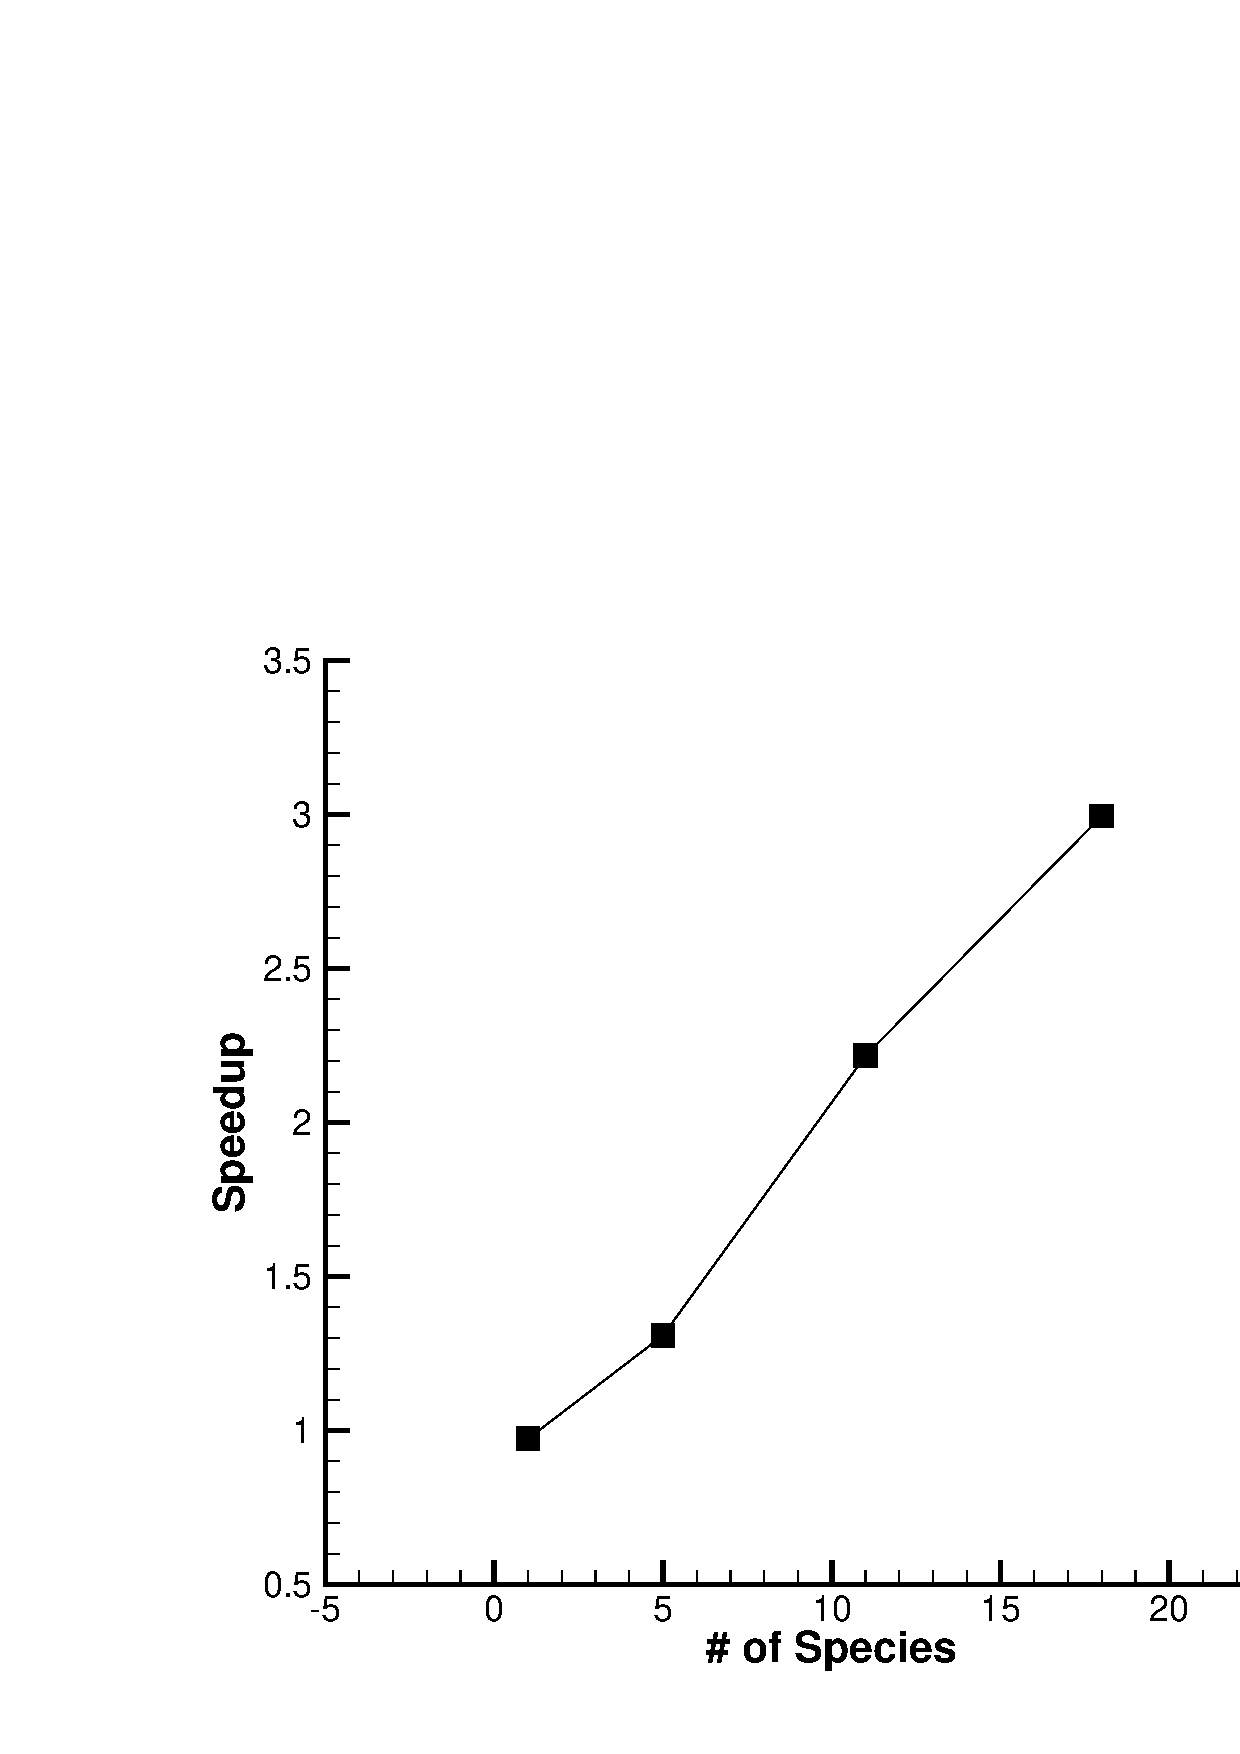
\includegraphics{total_cost}
\caption{Overall Relative Speedup of the Decoupled Scheme wrt the Fully Coupled Scheme}
\label{overall_speedup}
\end{center}
\end{figure}





\section{Conclusion}

The motivation for this work was to greatly increase the efficiency of the reacting gas flow solver path in FUN3D to aid in the development of an adjoint development for this path.  Because of the complexity of the high-energy physics and the large problem size associated with additional equations needed to preserve species mass, and this increased efficiency is extremely beneficial towards an adjoint formulation.  Most importantly, the decoupling of the species equations from the mixture equations is imperative in deriving sufficiently accurate jacobians for the Roe FDS scheme.  The 400\% decrease in memory required and 300\% speedup for the 18-species, at little to no cost of accuracy or stability, case clearly illustrates significant advantages of this method, at little to no cost of accuracy or stability.

\section*{A. Decoupled Flux Derivation}

For the Roe Flux Difference Splitting scheme, the species mass fluxes are given by:
%
\begin{equation}
	F_{\rho_s} = \frac{\rho_s^L\overline{U}^L+\rho_s^R\overline{U}^R}{2}
	-\frac{\tilde{c}_s(\lambda_1 dv_1 + \lambda_2 dv_2)+\lambda_3 dv_{3_s})}{2} \label{species_mass} \\
\end{equation}
\begin{align}	
		dv_1 &= \frac{p^R-p^L+\tilde{\rho} \tilde{a} (\overline{U}^R-\overline{U}^L)}{\tilde{a}^2} \\
		dv_2 &= \frac{p^R-p^L-\tilde{\rho} \tilde{a} (\overline{U}^R-\overline{U}^L)}{\tilde{a}^2} \\
		dv_{3_s} &= \frac{\tilde{a}^2 (\rho_s^R-\rho_s^L)- \tilde{c}_s (p^R-p^L)}{\tilde{a}^2}
\end{align}
\begin{align}
	\lambda_1 = \mid\mathbf{\overline{U}}+\tilde{a} \mid,\quad 
	\lambda_2 = \mid \mathbf{\overline{U}}-\tilde{a} \mid,\quad 
	\lambda_3 =  \mid \mathbf{\overline{U}} \mid
\end{align}
%
where the $\tilde{}$ notation signifies a roe-averaged quantity, given by:
%
\begin{gather}
	\mathbf{\tilde{U}} =w\mathbf{\tilde{U}}^L+(1-w)\mathbf{\tilde{U}}^R \\
	w = \frac{\tilde{\rho}}{\tilde{\rho}+\rho^R}
	%\mathbf{\tilde{U}}=\frac{\sqrt{\rho^L}\mathbf{U}^L + \sqrt{\rho^R}\mathbf{U}^R}{\sqrt{\rho^L}+\sqrt{\rho^R}}
\end{gather}
%
The species mass fluxes must sum to the total mass flux; thus, the total mixture mass flux is given as:
%
\begin{equation}
\label{total_mass}
	F_\rho = \sum\limits_{s}{F_{\rho_s}} = \frac{\rho^L\overline{U}^L+\rho^R\overline{U}^R}{2}
	-\frac{\tilde{c}_s(\lambda_1 dv_1 + \lambda_2 dv_2)+\lambda_3 dv_3)}{2}
\end{equation}
\begin{equation}
	dv_3 = \frac{\tilde{a}^2 (\rho^R-\rho^L)-(p^R-p^L)}{\tilde{a}^2}
\end{equation}
%
Multiplying eq.~(\ref{total_mass}) by the roe-averaged mass fraction and substituting into eq.~(\ref{species_mass}) results in:
%
\begin{equation}
\label{unsimp_sp_flux}
	F_{\rho_s} =\tilde{c}_s F_\rho + \frac{(c_s^L-\tilde{c}_s)\rho^L(\overline{U}^L+\mid \tilde{U}\mid)}{2}
	+ \frac{(c_s^R-\tilde{c}_s)\rho^R(\overline{U}^R-\mid \tilde{U}\mid)}{2}
\end{equation}
%
The notation can be further simplified by defining the normal velocities as follows:
%
\begin{equation}
\label{lambda_pm}
	\lambda^+ = \frac{\overline{U}^L+\mid \tilde{U}\mid}{2}, \quad 
	\lambda^- = \frac{\overline{U}^R-\mid \tilde{U}\mid}{2}
\end{equation}
%
Finally, substituting Eq.~(\ref{lambda_pm}) into Eq.~(\ref{unsimp_sp_flux}) yields the final result for calculating the species flux in decoupled system:
%
\begin{equation}
\label{sp_flux}
	F_{\rho_s} =\tilde{c}_s F_\rho + (c_s^L-\tilde{c}_s)\rho^L\lambda^+
	+ (c_s^R-\tilde{c}_s)\rho^R\lambda^-
\end{equation}
%
Form the convective contributions to the jacobians is straightforward.   Because the $\mathbf{U}'$ level variables are constant, only the left, right, and roe-averaged state mass fractions vary.  Differentiating Eq.~(\ref{sp_flux}) with respect to the mass fraction, $c_s$, the left and right state contributions are:
%
\begin{gather}
	\frac{\partial F_{\rho_s}}{\partial c^L_s} = wF_\rho+(1-w)\rho^L\lambda^+ - w\rho^R\lambda^- \\
	\frac{\partial F_{\rho_s}}{\partial c^R_s} = (1-w)F_\rho+(w-1)\rho^L\lambda^+ + w\rho^R\lambda^-
\end{gather}
%
Because there is no dependence between species in decoupled convective formulation, the jacobian block elements are purely diagonal for the convective contributions, of the form:
%
\begin{equation}
	\begin{pmatrix}
		\frac{\partial F_{\rho_1}}{\partial c_1} & & 0 \\
		 & \ddots &  \\
		 0 & & \frac{\partial F_{\rho_{ns}}}{\partial c_{ns}}
	\end{pmatrix}
\end{equation}

\section*{Acknowledgments}

The authors would like to recognize the FUN3D team at NASA Langley Research Center, for their support in integrating aspects of the compressible gas path into the reacting gas path of FUN3D.

%\begin{thebibliography}{9}% maximum number of references (for label width)
 %\bibitem{candler:82bk}
\bibliography{Abstract}
\bibliographystyle{plain}
%\end{thebibliography}

\end{document}

% - Release $Name:  $ -
